\subsection{SIGNS AND ASSEMBLIES}

The signs of a mathematical theory \(\mathcal{C}\)\footnote{The meaning of this expression will become clear as the chapter progresses.} are the following :

\begin{enumerate}
\def\labelenumi{(\arabic{enumi})}
\item
  The logical signs\footnote{For the intuitive meanings of these signs, see no. 3, Remark.}: \(\square, \tau, \vee, \neg\).
\item
  The letters.
\end{enumerate}

By letters we mean upper and lower case Roman letters, with or without accents. Thus A, A', A'', A''', \ldots{} are letters. At any place in the text it is possible to introduce letters other than those which have appeared in previous arguments.

\begin{enumerate}
\def\labelenumi{(\arabic{enumi})}
\setcounter{enumi}{2}
\tightlist
\item
  The specific signs, which depend on the theory under consideration.
\end{enumerate}

In the theory of sets we shall use only the following three specific signs: \(=, \in, \supset\) .

An assembly in \(\mathfrak{C}\) is a succession of signs of \(\mathfrak{C}\) written next to one another; certain signs, other than letters, may be joined in pairs by bars above the line, which are called links. *For example, in the Theory of Sets, in which \(\in\) is a specific sign,

\pandocbounded{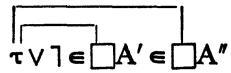
\includegraphics[keepaspectratio]{images/part001_434fa5c1de2e0e5711bd2657d8ea90475ca0e52e33fa2d57a405da317d612ec5.jpg}}

is an assembly.*

The exclusive use of assemblies would lead to insuperable difficulties both for the printer and for the reader. For this reason current texts use abbreviating symbols (notably words of ordinary speech) which do not belong to formal mathematics. The introduction of such symbols is the object of definitions. Their use is not indispensable to the theory, and can often lead to confusion which only a certain familiarity with the subject will enable the reader to avoid.

\minorheading{Examples}

\begin{enumerate}
\def\labelenumi{(\arabic{enumi})}
\item
  The assembly \(\vee\neg\) is represented by \(\Longrightarrow\) .
\item
  The following symbols represent assemblies (and very long ones at that):
\end{enumerate}

\[
\begin{gathered}
\text{``3 and 4''} \\
\phi \\
\mathbf{N} \\
\mathbf{Z} \\
\text{``the real line''} \\
\text{``the }\Gamma\text{ function''} \\
f \circ g \\
\pi = \sqrt{2} + \sqrt{3} \\
1 \in 2
\end{gathered}
\]

``Every finite division ring is a field''

``The zeros of \(\zeta(s)\) other than \(-2, -4, -6, \ldots\) lie on the line

\[
\mathcal{R}(s) = 1/2
\]''.

In general, the symbol used to represent an assembly contains all the letters which appear in the assembly. Nevertheless, this principle can sometimes be infringed without risk of confusion. *For example, ``the completion of X'' represents an assembly which contains the letter X, but which also contains the letter which represents the set of entourages of the uniform structure of X. On the other hand,

\[
\int_ {0} ^ {1} f (x) d x
\]

represents an assembly in which the letter x (and the letter d) do not appear; and the assemblies represented by N, Z, ``the Γ function'' do not contain any letters.*

A mathematical theory (or simply a theory) contains rules which allow us to assert that certain assemblies of signs are terms or relations of the theory, and other rules which allow us to assert that certain assemblies are theorems of the theory.

The description of these rules, which will appear in this chapter, does not belong to formal mathematics; the rules involve assemblies which are more or less undetermined, for example undetermined letters. To simplify the exposition it is convenient to denote such assemblies by less cumbersome symbols. We shall use, especially, combinations of signs (of a mathematical theory), bold-face italic letters (with or without indices or accents), and particular symbols, of which some examples will be given. Since our object is only to avoid circumlocutions (cf.~note (*), § 3, no. 1, p.~28) we shall not enunciate strict general rules for the use of these symbols; the reader will be able to reconstruct without trouble the assembly in question, in each particular case. By abuse of language we shall often say that the symbols are assemblies, rather than that they denote assemblies: expressions such as ``the assembly A'' or ``the letter x'', in the statements of the following rules, should therefore be replaced by ``the assembly denoted by A'' or ``the letter denoted by x''.

Let \(A\) and \(B\) be assemblies. We shall denote by \(AB\) the assembly obtained by writing the assembly \(B\) on the right of the assembly \(A\) . We shall denote by \(\vee A \neg B\) the assembly obtained by writing, from left to right, the sign \(\vee\) , the assembly \(A\) , the sign \(\neg\) , the assembly \(B\) . And so on.

Let \(A\) be an assembly and let \(x\) be a letter. We shall denote by \(\tau_{x}(A)\) the assembly constructed as follows: form the assembly \(\tau A\) , link each occurrence of \(x\) in \(A\) to the \(\tau\) written on the left of \(A\) , and then replace \(x\) everywhere it occurs by the sign \(\square\) . The assembly denoted by \(\tau_{x}(A)\) therefore does not contain \(x\) .

Example. The symbol \(\tau_{x}(\in xy)\) represents the assembly

\[
\tau \in \square y.
\]

Let A and B be assemblies and let x be a letter. The assembly obtained by replacing x, wherever it occurs in A, by the assembly B is denoted by \((B|x)A\) (read: B replaces x in A). If x does not appear in A, then \((B|x)A\) is identical with A; in particular,

\[
(B | \boldsymbol {x}) \tau_ {\boldsymbol {x}} (A)
\]

is identical with \(\tau_{\mathbf{x}}(A)\) .

Example. If we replace \(x\) by \(\square\) wherever \(x\) occurs in the assembly \(\vee \in xy = xx\) , we obtain the assembly \(\vee \in \square y = \square \square\) .

If \(A\) is an assembly and we are interested particularly in a letter \(x\) , or two distinct letters \(x\) and \(y\) (which may or may not appear in \(A\) ), we shall often write \(A \{x\}\) or \(A \{x, y\}\) . In this case we write \(A \{B\}\) instead of \((B|x)A\) . We denote by \(A \{B, C\}\) the assembly obtained by simultaneously replacing \(x\) by \(B\) and \(y\) by \(C\) wherever they occur in \(A\) (note that \(x\) and \(y\) may appear in \(B\) and in \(C\) ); if \(x'\) and \(y'\) are distinct letters, other than \(x\) and \(y\) , which appear in neither \(A, B\) , nor \(C\) , then \(A \{B, C\}\) is the same as \((B|x') (C|y') (x'|x) (y'|y)A\) .

Remark. When an abbreviating symbol \(\Sigma\) is introduced, by means of a definition, to represent a certain assembly, the (usually tacit) convention is made of representing the assembly obtained by substituting an assembly B for a letter x in the original assembly, by the symbol obtained by the replacing the letter x in \(\Sigma\) by the assembly B (or, more often, by an abbreviating symbol representing the assembly B).

¶ *For example, having defined what assembly is represented by the symbol E⊗F, where E and F are letters --- an assembly which, incidentally, contains other letters besides E and F --- the symbol Z⊗F can be used without further explanation.*

¶ This rule can lead to confusions, which are avoided by the use of various typographical devices; the most common consists in replacing x by (B) in place of B.

¶ *For example, M∩N denotes an assembly containing the letter N. If we substitute for N the assembly represented by P∪Q, we get an assembly denoted by M∩(P∪Q).*

